\chapter{Habitat of ice reservoirs}

AIRs cannot be built anywhere. They require sufficient water supply, specific topography and favourable weather
conditions to amass a seasonal stock of ice. In this chapter, we attempt to quantify these requirements by
examining the magnitude of these differences across the AIRs built in India and Switzerland. We also discuss
strategies to judge the utility of AIRs in new locations.

\section{Requirements for AIR construction}

\subsection{Water supply}

The water source of an AIR could be either a spring or a stream. Springs are the ideal water source since they
are easy to transport via pipelines to the construction site due to their relatively warm temperatures. Other
water sources have higher risks of freezing events in the fountain pipeline.

\subsection{Weather conditions}

AIRs prefer colder, drier and less-cloudy regions. Correspondingly, temperature, humidity and number of
cloud-free days during the construction period can be used to rank different sites. 

However, determining favourable construction locations is challenging due to the significant interannual,
interregional and intraregional variations in weather conditions.

\subsubsection{Interannual variability}

Fig. \ref{fig:CH_diffs} (a) shows the correlation of the ice volume changes with median temperature during
January for AIRs built in the Swiss locations across three winters . Contrary to expectations, ice volume
increases as median temperature increases. This indicates that temperature is not the primary driver of
interannual variations in the ice volume. Instead, we found that  higher wind speeds drove the volume
differences of these AIRs due to wind driven redistribution effects (see paper III). The influence of this
process on the spray radius managed to generate AIRs six times bigger in spite of temperatures being 3 $\degree
C$ warmer (see Fig. \ref{fig:CH_diffs} (b)). 

\begin{figure}[t]
\centering
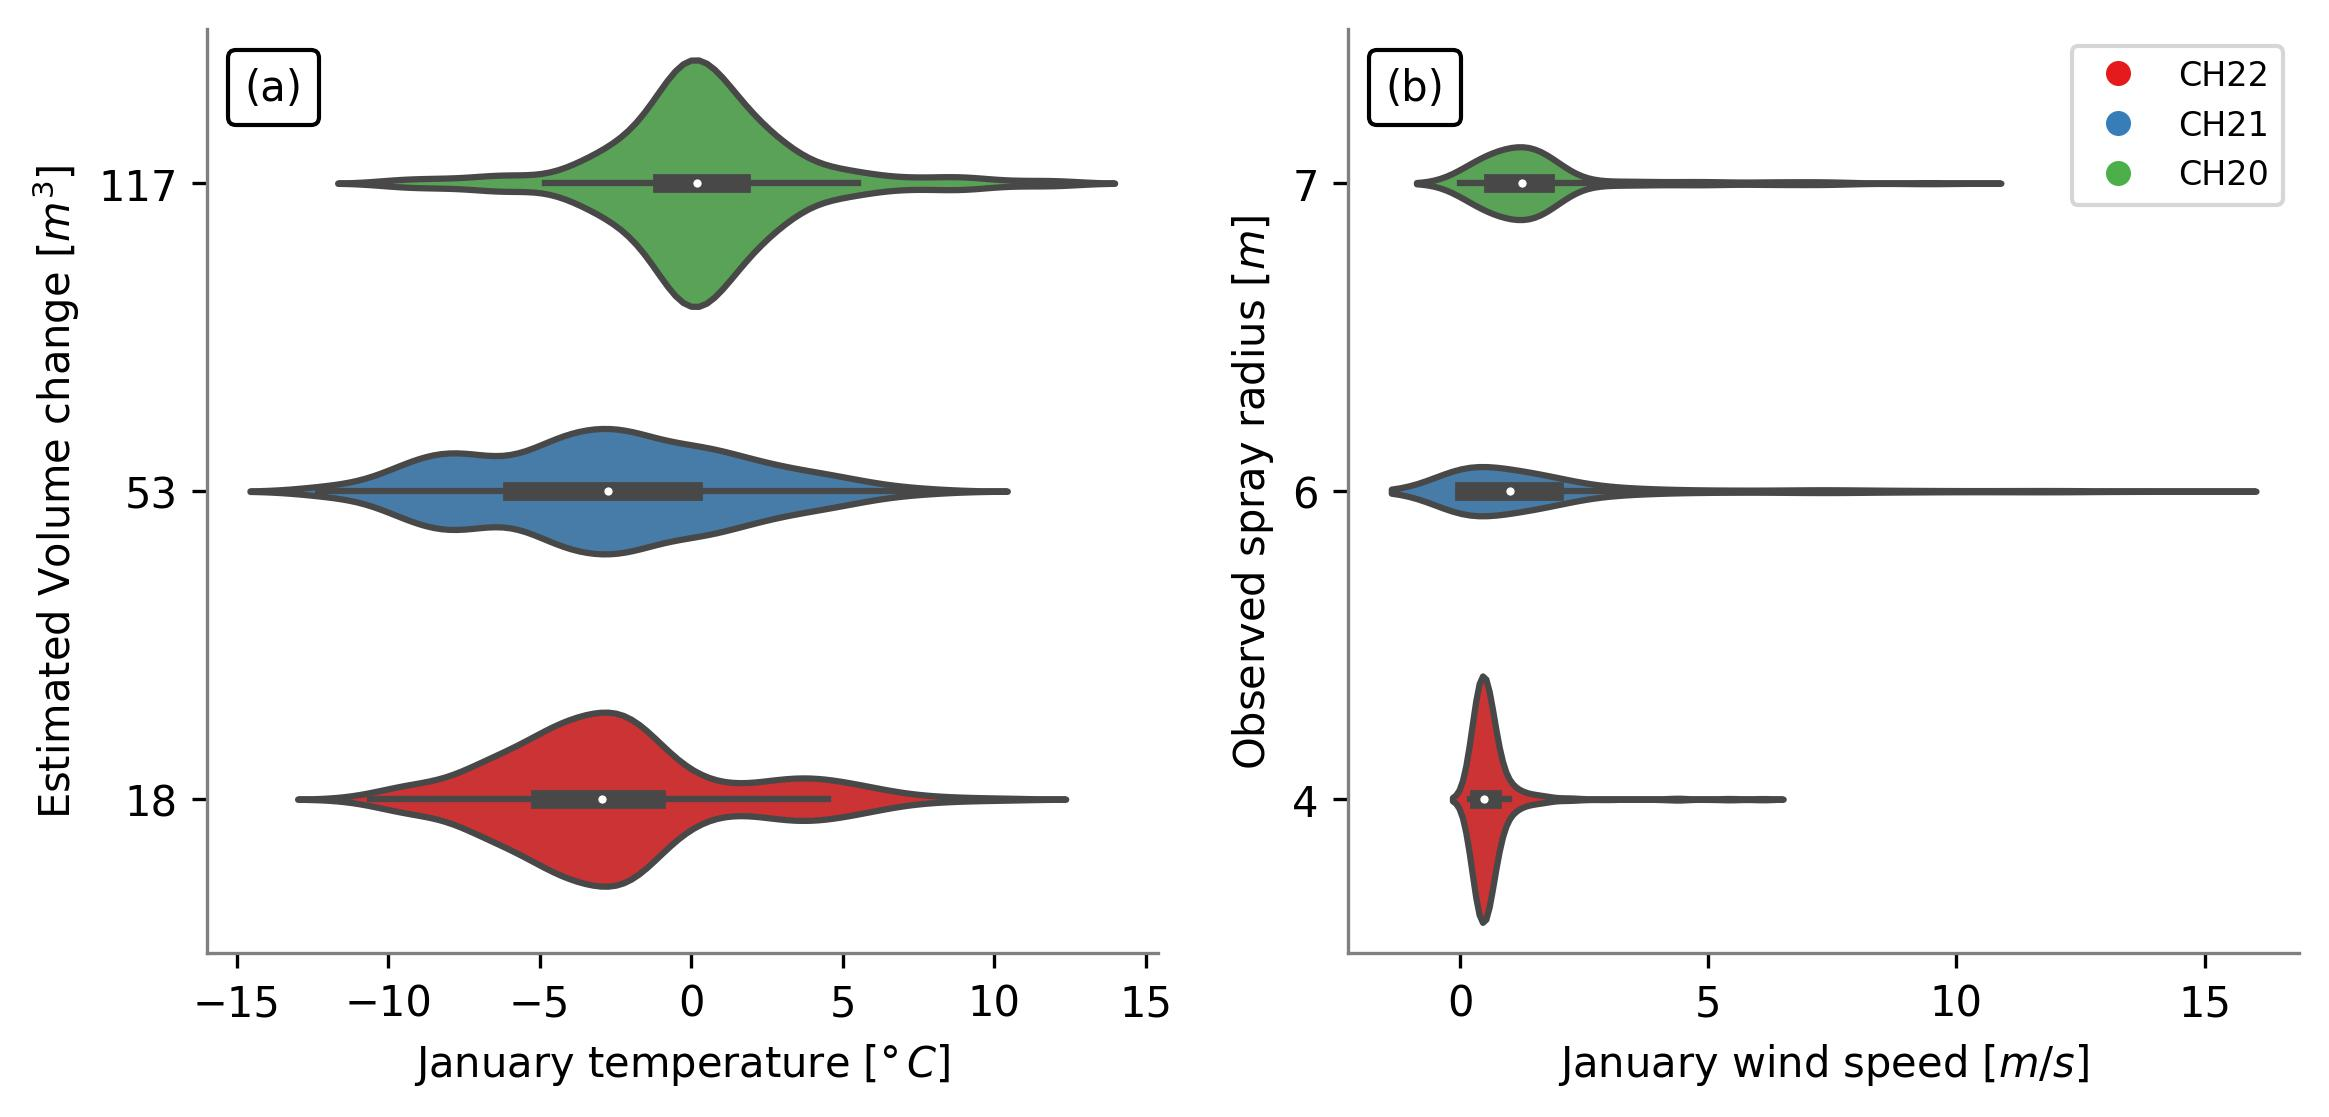
\includegraphics[width=\textwidth]{figs/CH_diffs.jpg}
\caption{(a) Estimated volume change and median temperature and (b) Observed spray radius and median wind speed
during january for AIRs built across three winters. } 
\label{fig:CH_diffs}
\end{figure}

\subsubsection{Interregional variability}

\begin{figure}[t]
\centering
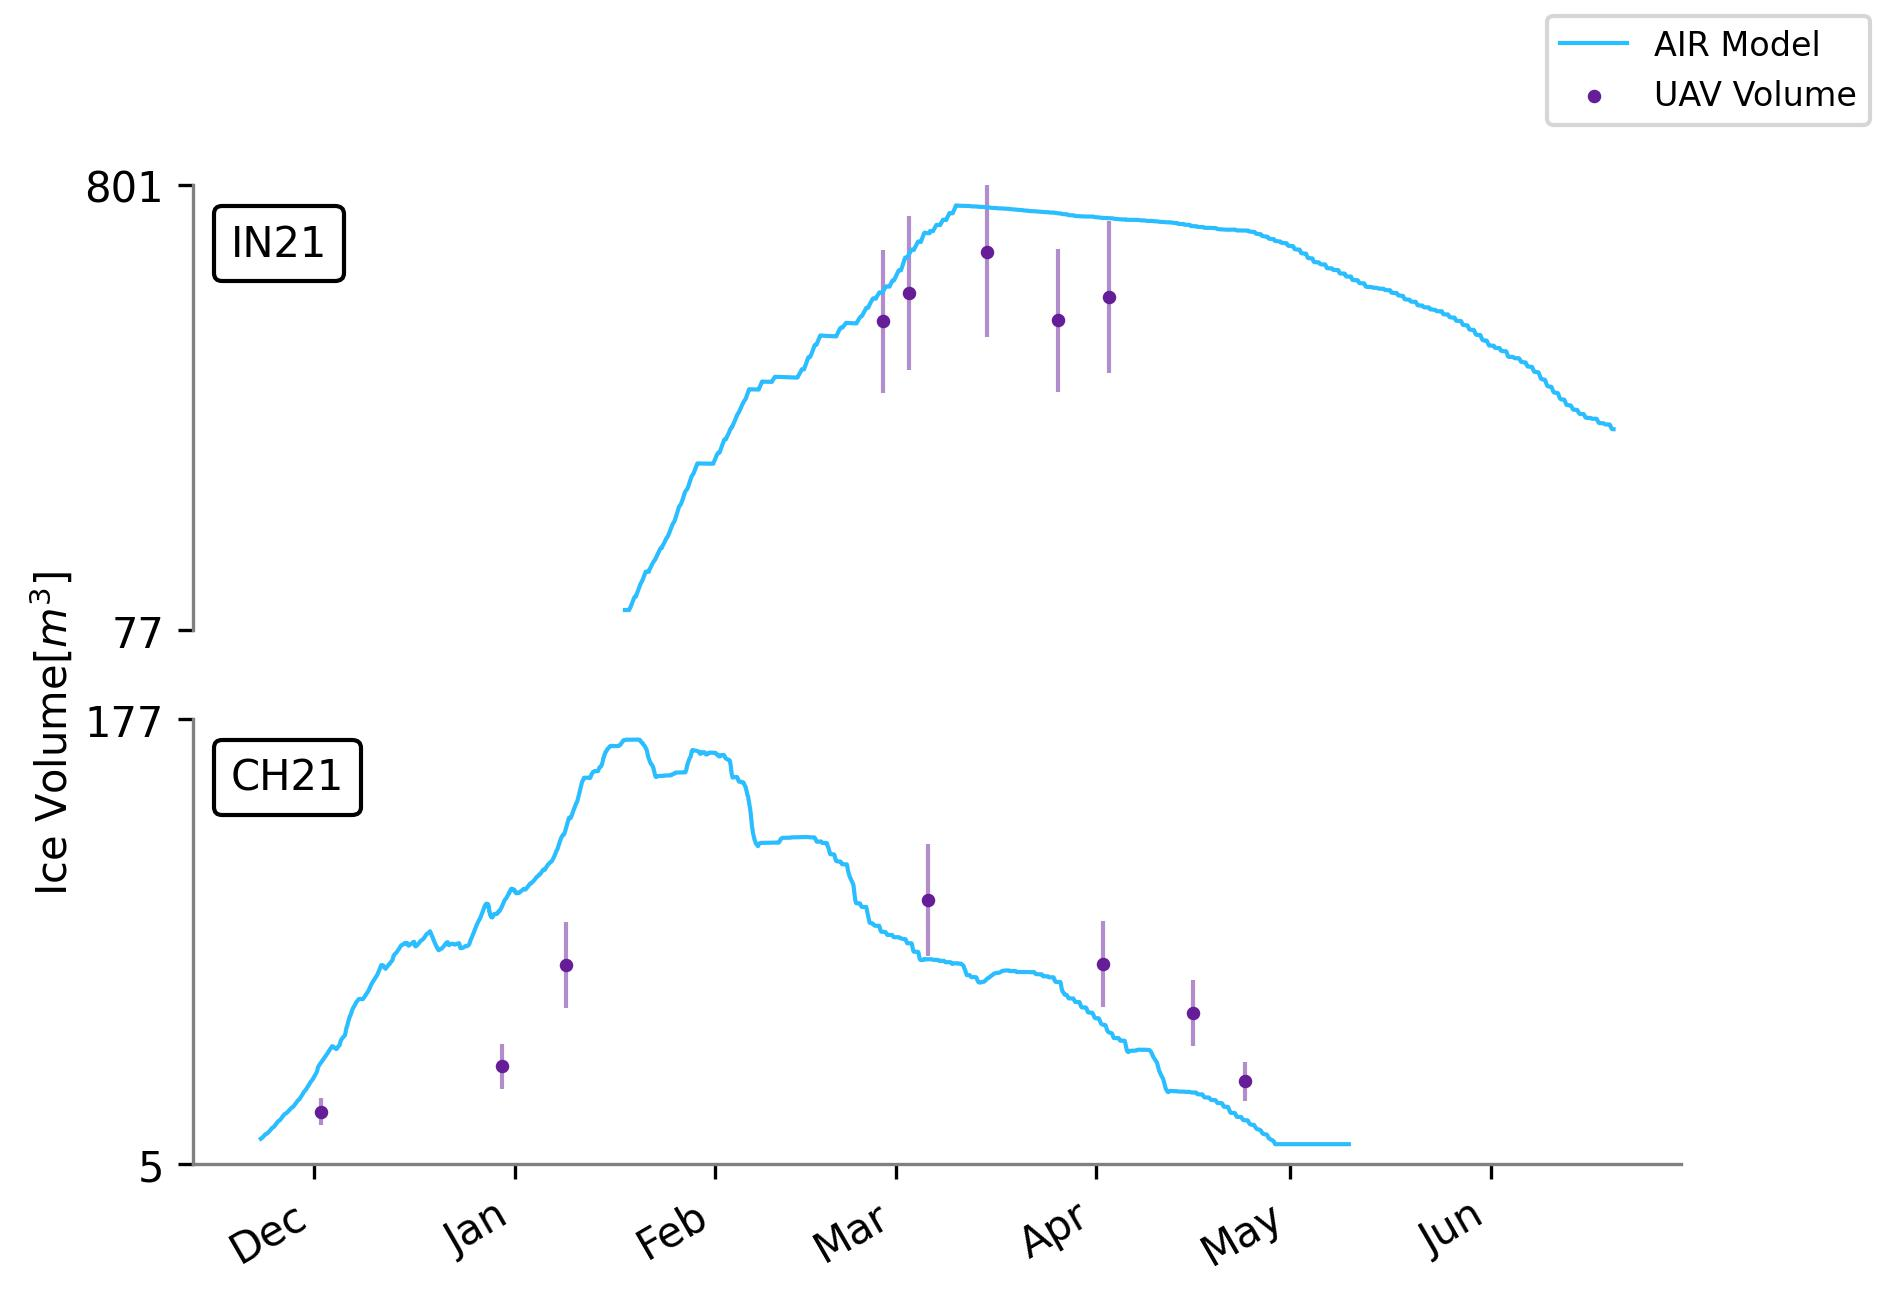
\includegraphics[width=12cm]{figs/IN21vsCH21.jpg}
\caption{AIRs show significant variation in volume evolution depending on the choice of construction location.}
\label{fig:2AIRs}
\end{figure}

\subsubsection{Intraregional variability}

\begin{figure}[t]
\centering
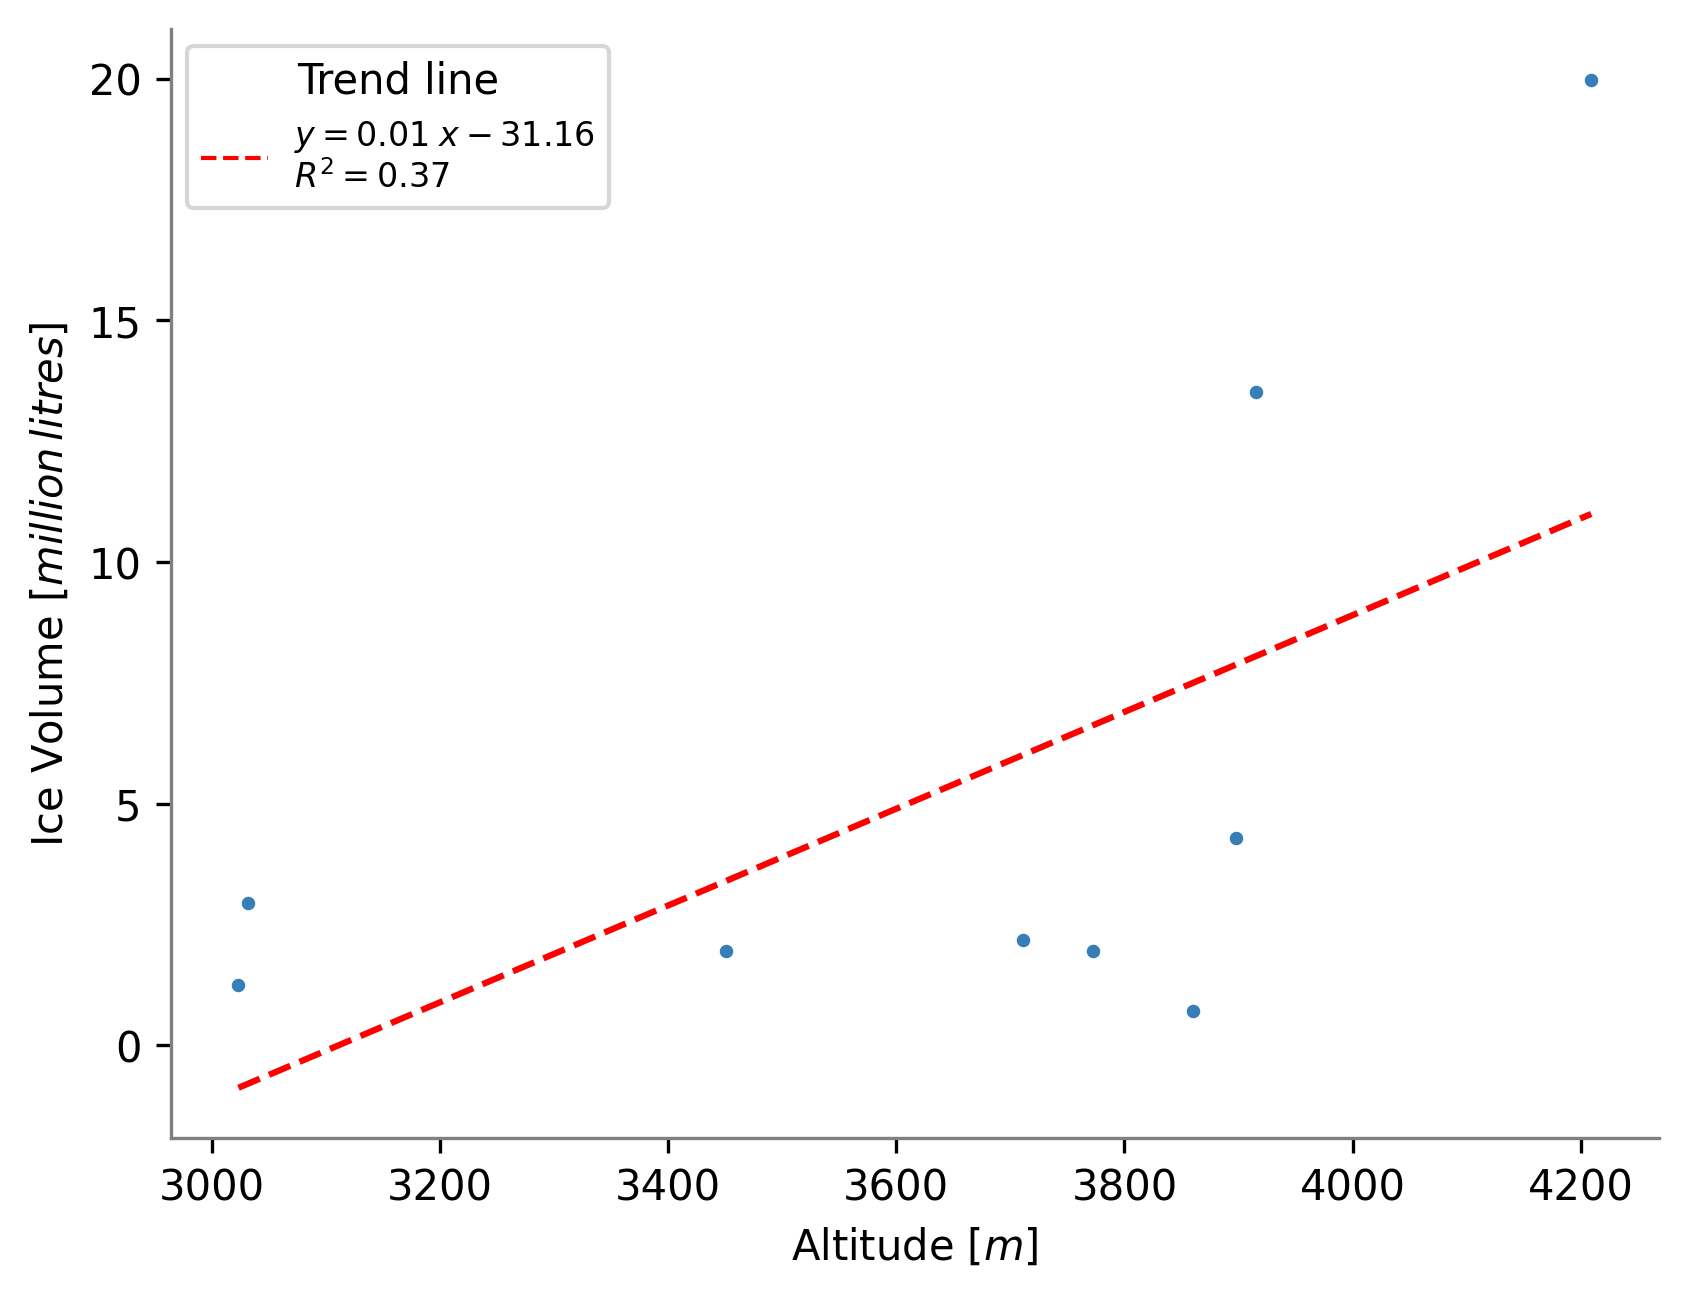
\includegraphics[width=12cm]{figs/altitudevsvolume.png}
\caption{(a) Estimated volume change and median temperature and (b) Observed spray radius and median wind speed
during january for AIRs built across three winters. }
\label{fig:altitudevsvolume}
\end{figure}



\subsection{Topography}

AIRs prefer shadowed valleys. This is because these landforms have lower sunshine hours which is the major
driver of the melting rate of all the AIRs studied in this thesis.

\subsection{Checklist to identify AIR construction regions}

Accordingly, we propose the following checklist to determine AIR site suitability. The values presented are
determined based on past construction experiences and can be used as guidelines to avoid construction attempts
in unfavourable sites.

\begin{enumerate}

  \item Minimum mean monthly temperature less than $0 \degree C$. 
  \item Water supply with mean discharge rate more than $2 l/min$. 
  \item Terrain slope between water source and site greater than 10 m every km. 

\end{enumerate}

\subsection{Metrics to rank sites within the same region }

Given a valley or a region satisfying the above requirements, further selection of sites around the particular
water supply can be performed using the criterions below: 

\begin{enumerate}
  \item Water source temperature is higher.
  \item Daylight hours are lower due to shadows.
  \item Altitude is higher.
\end{enumerate}

Such villages are expected to produce AIRs that supply daily meltwater in the order of thousands of litres for 2
months. 

Different forms of AIRs show different sensitivities to each of these requirements. This is discussed in the
next chapter.

% \begin{itemize}
%   \item {\bf Water supply} : The water source of an AIR could be either a spring or a stream. Springs are the ideal
%     water source since they are easy to transport via pipelines to the construction site due to their relatively
%     warm temperatures. Other water sources have higher risks of pipeline freezing events. 

%   \item {\bf Weather conditions} : AIRs prefer colder, drier and less-cloudy regions. Correspondingly,
%     temperature, humidity and number of cloud-free days during the construction period can be used to rank
%     different sites. 

%   \item {\bf Topography} : AIRs prefer shadowed valleys. This is because these landforms have lower sunshine
%     hours which is the major driver of the melting rate of all the AIRs studied in this thesis.

% \end{itemize}

% This imposes several meteorological and topographical requirements for the chosen
% construction location. The meteorological requirements can be used to identify favourable regions worldwide
% whereas the topographical requirements can be used to pinpoint the construction site within the respective
% region. Below we detail these requirements and propose methodologies for finding construction sites satisfying
% them. 
  % \item Daylight hours are lower.
  % \item Cloudy days are lower.
  % \item Temperature is lower.
  % \item Humidity is lower.

% The ice reservoir technology has found limited adoption in regions beyond Ladakh. However, this

% It remains to be seen where else AIRs can be of utility.

% AIRs cannot be built anywhere. They require weather conditions cold enough to amass a seasonal stock of ice. The
% weather suitability of locations can be identified using the model developed in paper I. But such a methodology
% has a data requirement often incompatible with what is available. Reanalysis datasets like ERA5 can serve as 

% The utility of AIRs depends on their daily meltwater discharge. 

% Temperature based 
